%==========================================================================
% APPENDICES
%==========================================================================
\chapter{Data Dictionary}\label{app:data}

\paragraph{Douala charts} One row per reading, transcribed by hand from the ward observation charts without names (\cref{tab:dict-douala}). The file is not published.

\begin{table}[htbp]
\centering\footnotesize
\caption{Columns of the Douala charts file.}\label{tab:dict-douala}
\begin{tabularx}{\textwidth}{@{}>{\ttfamily\raggedright\arraybackslash}p{2.5cm} >{\raggedright\arraybackslash}X >{\raggedright\arraybackslash}p{4.6cm}@{}}
\toprule
\normalfont\textbf{Column} & \textbf{Content} & \textbf{Use} \\
\midrule
patient & integer code assigned at transcription & grouping of the samples \\
age, sex & years; F or M & features; subgroups; ages grouped in five-year bands before sharing \\
height\_cm, weight\_kg & empty in every row & not used \\
date & date of the reading & time since the patient's first reading \\
time & M (morning) or S (evening, \emph{soir}) & slot; the two slots are placed 12~h apart \\
sbp, dbp & systolic and diastolic pressure, mmHg & channels \\
hr & pulse, beats per minute & channel \\
glucose\_gl & capillary glucose as written on the chart, g/L & source of the glucose channel \\
glucose & glucose in mmol/L, from g/L with 18.0156~mg/dL per mmol/L & channel \\
glucose\_state & meal status; \emph{casuel} (random) in every row & not used: in-hospital thresholds do not depend on it \\
notes & free text, 5 rows & not used \\
label & level under the earlier unsourced rule & comparison of the two rules only (\cref{tab:rule-change}) \\
\bottomrule
\end{tabularx}
\end{table}

\paragraph{eICU demonstration subset} Version 2.0.1 \parencite{eicudemo}, checked against its published checksums before every run. \Cref{tab:dict-eicu} lists the tables and columns read. A stay is eligible when the patient is an adult and hypertension or diabetes is recorded in the diagnoses or the past history; hypertensions of another nature (pulmonary, intracranial, portal, ocular, intra-abdominal, gestational) are excluded.

\begin{table}[htbp]
\centering\footnotesize
\caption{Tables and columns of eICU used.}\label{tab:dict-eicu}
\begin{tabularx}{\textwidth}{@{}>{\ttfamily\raggedright\arraybackslash}p{2.6cm} >{\ttfamily\raggedright\arraybackslash}X >{\raggedright\arraybackslash}p{4.6cm}@{}}
\toprule
\normalfont\textbf{Table} & \normalfont\textbf{Columns} & \textbf{Use} \\
\midrule
patient & patientunitstayid, uniquepid, hospitalid, age, gender & stays, patients, hospitals; age and sex \\
diagnosis & diagnosisstring & eligibility \\
pastHistory & pasthistorypath & eligibility \\
vitalAperiodic & noninvasivesystolic, noninvasivediastolic, observationoffset & cuff pressure at each slot \\
vitalPeriodic & heartrate, observationoffset & pulse at each slot \\
lab & labname (bedside glucose), labresult, labresultoffset & glucose at each slot, mg/dL to mmol/L \\
\bottomrule
\end{tabularx}
\end{table}

\chapter{Benchmark Configuration}\label{app:config}

The benchmark is declared in \texttt{configs/benchmark.yaml} of the research package before any run (\cref{tab:search-spaces}). Window length and class weights are searched for every candidate; the number of configurations tried per candidate and outer fold is fixed. Seed 20261019; five outer folds grouped by hospital, four inner folds grouped by patient, three repeats.

\begin{table}[htbp]
\centering\footnotesize
\caption{Search spaces and number of configurations. Ranges marked log are searched on a logarithmic scale.}\label{tab:search-spaces}
\begin{tabularx}{\textwidth}{@{}>{\raggedright\arraybackslash}p{2.7cm} c >{\raggedright\arraybackslash}X >{\raggedright\arraybackslash}X@{}}
\toprule
\textbf{Candidate} & \textbf{Trials} & \textbf{Structural} & \textbf{Training} \\
\midrule
All & -- & window 24, 48, 72, 96~h & class weights none or balanced \\
Ordinal logistic & 15 & -- & $C \in [10^{-3}, 10^{2}]$, log \\
PCA + ordinal logistic & 15 & components 1--8 & $C \in [10^{-3}, 10^{2}]$, log \\
Random forest & 20 & max features $\sqrt{p}$, 0.5, 1.0; min leaf 1--50, log; depth 3, 6, 12, none & -- \\
CatBoost & 25 & depth 2--8; iterations 100--1\,000, log & learning rate 0.01--0.3, log; L2 1--30, log \\
Value forecast, ridge & 15 & -- & $\alpha \in [10^{-3}, 10^{3}]$, log \\
Value forecast, CatBoost & 25 & as CatBoost & as CatBoost \\
GRU-D & 20 & hidden units 4, 8, 16, 32 & dropout 0--0.5; learning rate $10^{-3}$--0.03, log; weight decay $10^{-6}$--$10^{-2}$, log; auxiliary loss weight 0--1 \\
Masked LSTM & 20 & hidden units 4, 8, 16, 32; layers 1, 2 & as GRU-D \\
\bottomrule
\end{tabularx}
\end{table}

\paragraph{Rerunning the results} From \texttt{telemonitor-research}, every number and figure of the thesis is produced by a script (\cref{tab:scripts}).

\begin{table}[htbp]
\centering\footnotesize
\caption{Scripts of the research package and what they produce.}\label{tab:scripts}
\begin{tabularx}{\textwidth}{@{}>{\ttfamily\raggedright\arraybackslash}p{5.1cm} X@{}}
\toprule
\normalfont\textbf{Script} & \textbf{Produces} \\
\midrule
01\_douala\_audit.py & cohort description, quality flags, terminal digits, label uncertainty (\cref{sec:results-data}) \\
02\_label\_rules.py & the earlier rule against the sourced rule (\cref{tab:rule-change}) \\
04\_sample\_size.py & criteria of Riley et al.\ for both datasets (\cref{tab:sample-size}) \\
05\_eicu\_cohort.py & eligibility, harmonisation and samples of eICU \\
06\_benchmark.py & nested benchmark and external validation; resumes after an interruption \\
07\_app\_parity\_fixture.py & the fixture replayed by the application's parity tests \\
08\_figures.py; 13\_results\_tables.py & figures and tables of a saved run \\
09\_kappa\_sample\_size.py & size of the physician's relabelling \\
10\_sensitivity\_flags\_slots.py & shrinkage constant and slot tolerance (\cref{tab:tolerance}) \\
11\_export\_model.py & the model served by the risk service \\
12\_state\_comparison.py & benchmark of the measures of state evolution \\
14\_thesis\_data\_figures.py & data of \cref{fig:douala-timeline,fig:values,fig:transitions} \\
\bottomrule
\end{tabularx}
\end{table}

\chapter{Record Schema}\label{app:schema}

The fields of a reading and of an event in Cloud Firestore (\cref{fig:data-model}). The security rules validate every field on the server.

\begin{table}[htbp]
\centering\footnotesize
\caption{Fields of a reading, \texttt{users/\{uid\}/readings/\{id\}}.}\label{tab:schema-reading}
\begin{tabularx}{\textwidth}{@{}>{\ttfamily\raggedright\arraybackslash}p{3.4cm} >{\raggedright\arraybackslash}p{2.1cm} X@{}}
\toprule
\normalfont\textbf{Field} & \textbf{Type} & \textbf{Meaning} \\
\midrule
recordedAt & time & measurement time stated by the patient, at most 30 days before arrival \\
timestamp & time & arrival time, set by the server \\
entryMode & text & manual (Bluetooth entry is specified, not built) \\
sbp, dbp, hr & numbers & retained reading of the protocol pair; mmHg and beats per minute \\
glucose, context & number; text & mmol/L; fasting, before a meal, after a meal or random, required with glucose \\
readingCount & number & 1 or 2 readings in the session \\
firstSbp, firstDbp, firstHr & numbers & first reading of the pair, kept for audit \\
supersedes & reference & the reading this one corrects \\
notes & text & free text of the patient \\
qualityFlag & text & set by the worker: ok, out\_of\_range, unit\_suspect, duplicate, carried\_forward, extreme \\
\bottomrule
\end{tabularx}
\end{table}

\begin{table}[htbp]
\centering\footnotesize
\caption{Fields of an event, \texttt{users/\{uid\}/events/\{id\}}.}\label{tab:schema-event}
\begin{tabularx}{\textwidth}{@{}>{\ttfamily\raggedright\arraybackslash}p{3.4cm} >{\raggedright\arraybackslash}p{2.1cm} X@{}}
\toprule
\normalfont\textbf{Field} & \textbf{Type} & \textbf{Meaning} \\
\midrule
patientId, clinicianId & references & the patient and the assigned clinician \\
triggerSource & text & rule, model or non\_transmission \\
tier, score & text; number & yellow or red; the model's probability when the model raised it \\
readingId, trigger & reference; map & the triggering reading and values, or the profile and its means \\
thresholdVersion, modelVersion & text & versions in force when the event was raised \\
tsTriggered, status & time; text & creation; open or closed \\
verdict, action, comment & text & confirmed, not\_significant or uncertain; none, advice, treatment\_change, consultation or referral \\
tsReviewed, reviewedBy & time; reference & closure of the event, once \\
escalatedAt, escalatedTo & time; reference & escalation to the named alternate \\
\bottomrule
\end{tabularx}
\end{table}

\chapter{Application Screens}\label{app:screens}

\noindent\begin{minipage}{\textwidth}
\captionsetup{type=figure}
\centering
\begin{subfigure}[t]{0.17\textwidth}\centering
  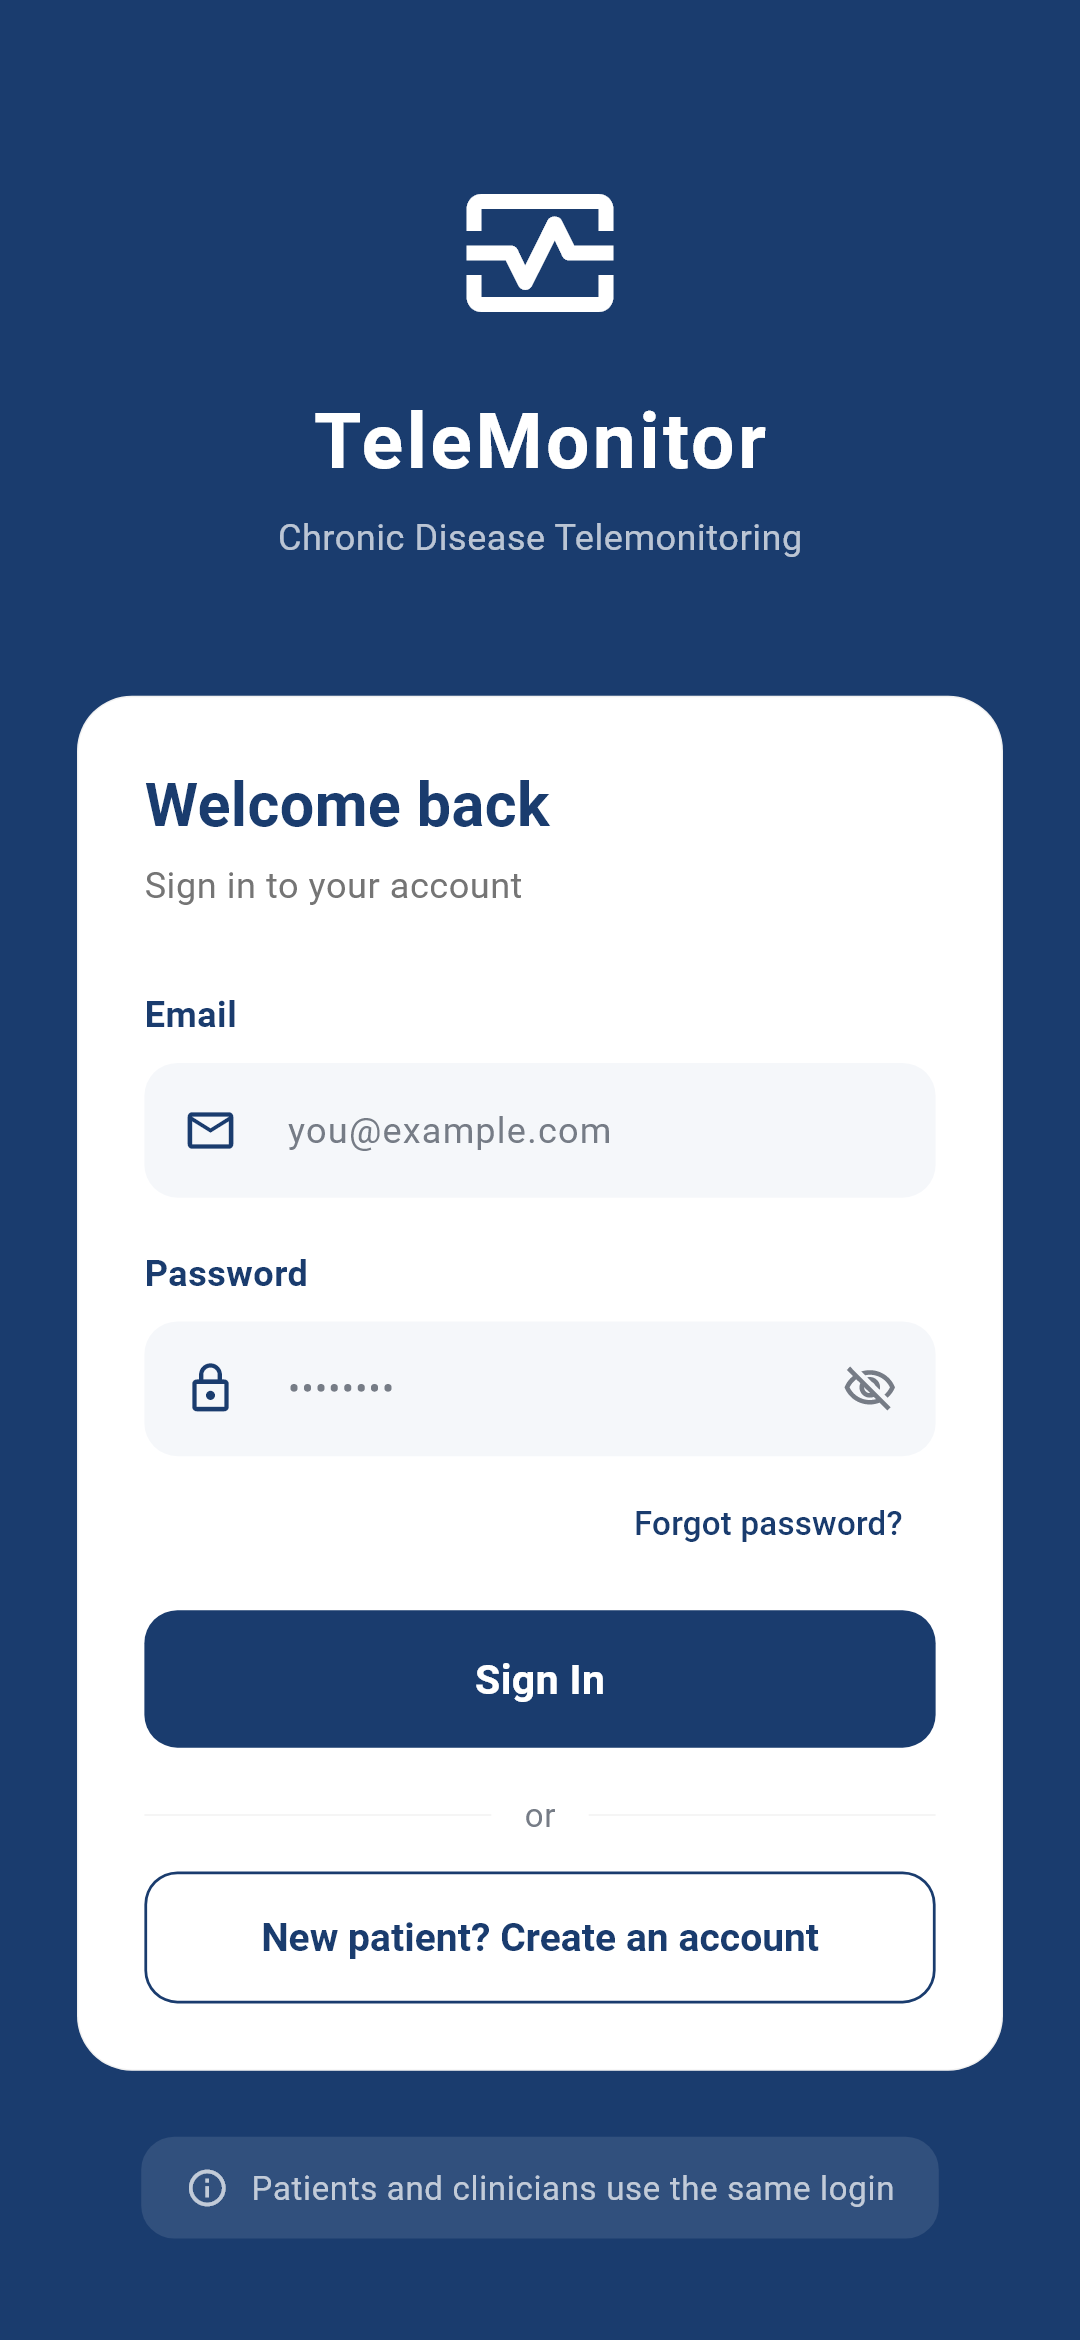
\includegraphics[width=\linewidth]{figures/screens/login_light.png}
  \caption{Sign-in}
\end{subfigure}\hfill
\begin{subfigure}[t]{0.17\textwidth}\centering
  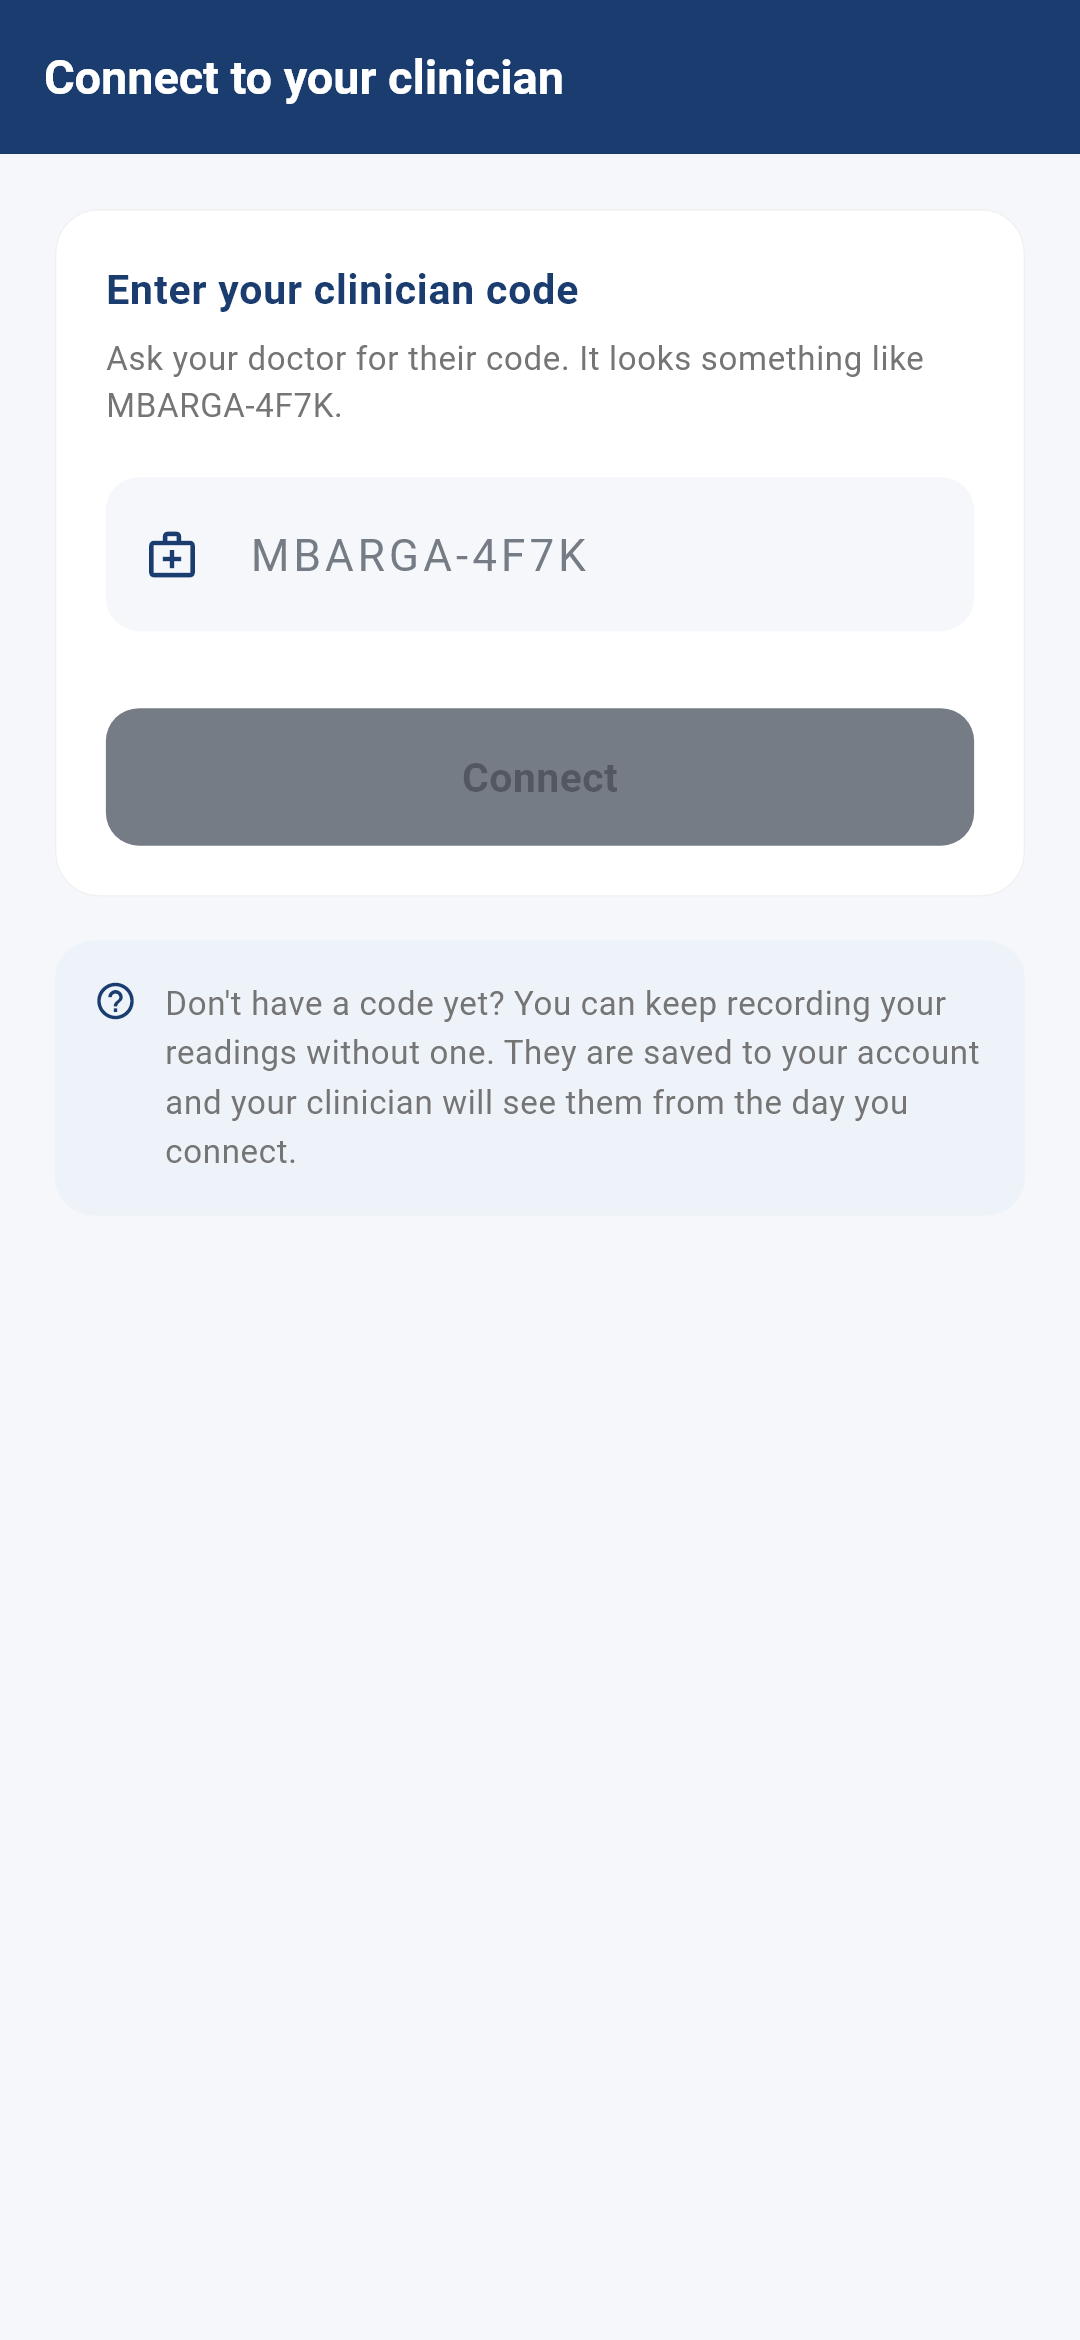
\includegraphics[width=\linewidth]{figures/screens/connect_clinician_light.png}
  \caption{Enrolment}
\end{subfigure}\hfill
\begin{subfigure}[t]{0.17\textwidth}\centering
  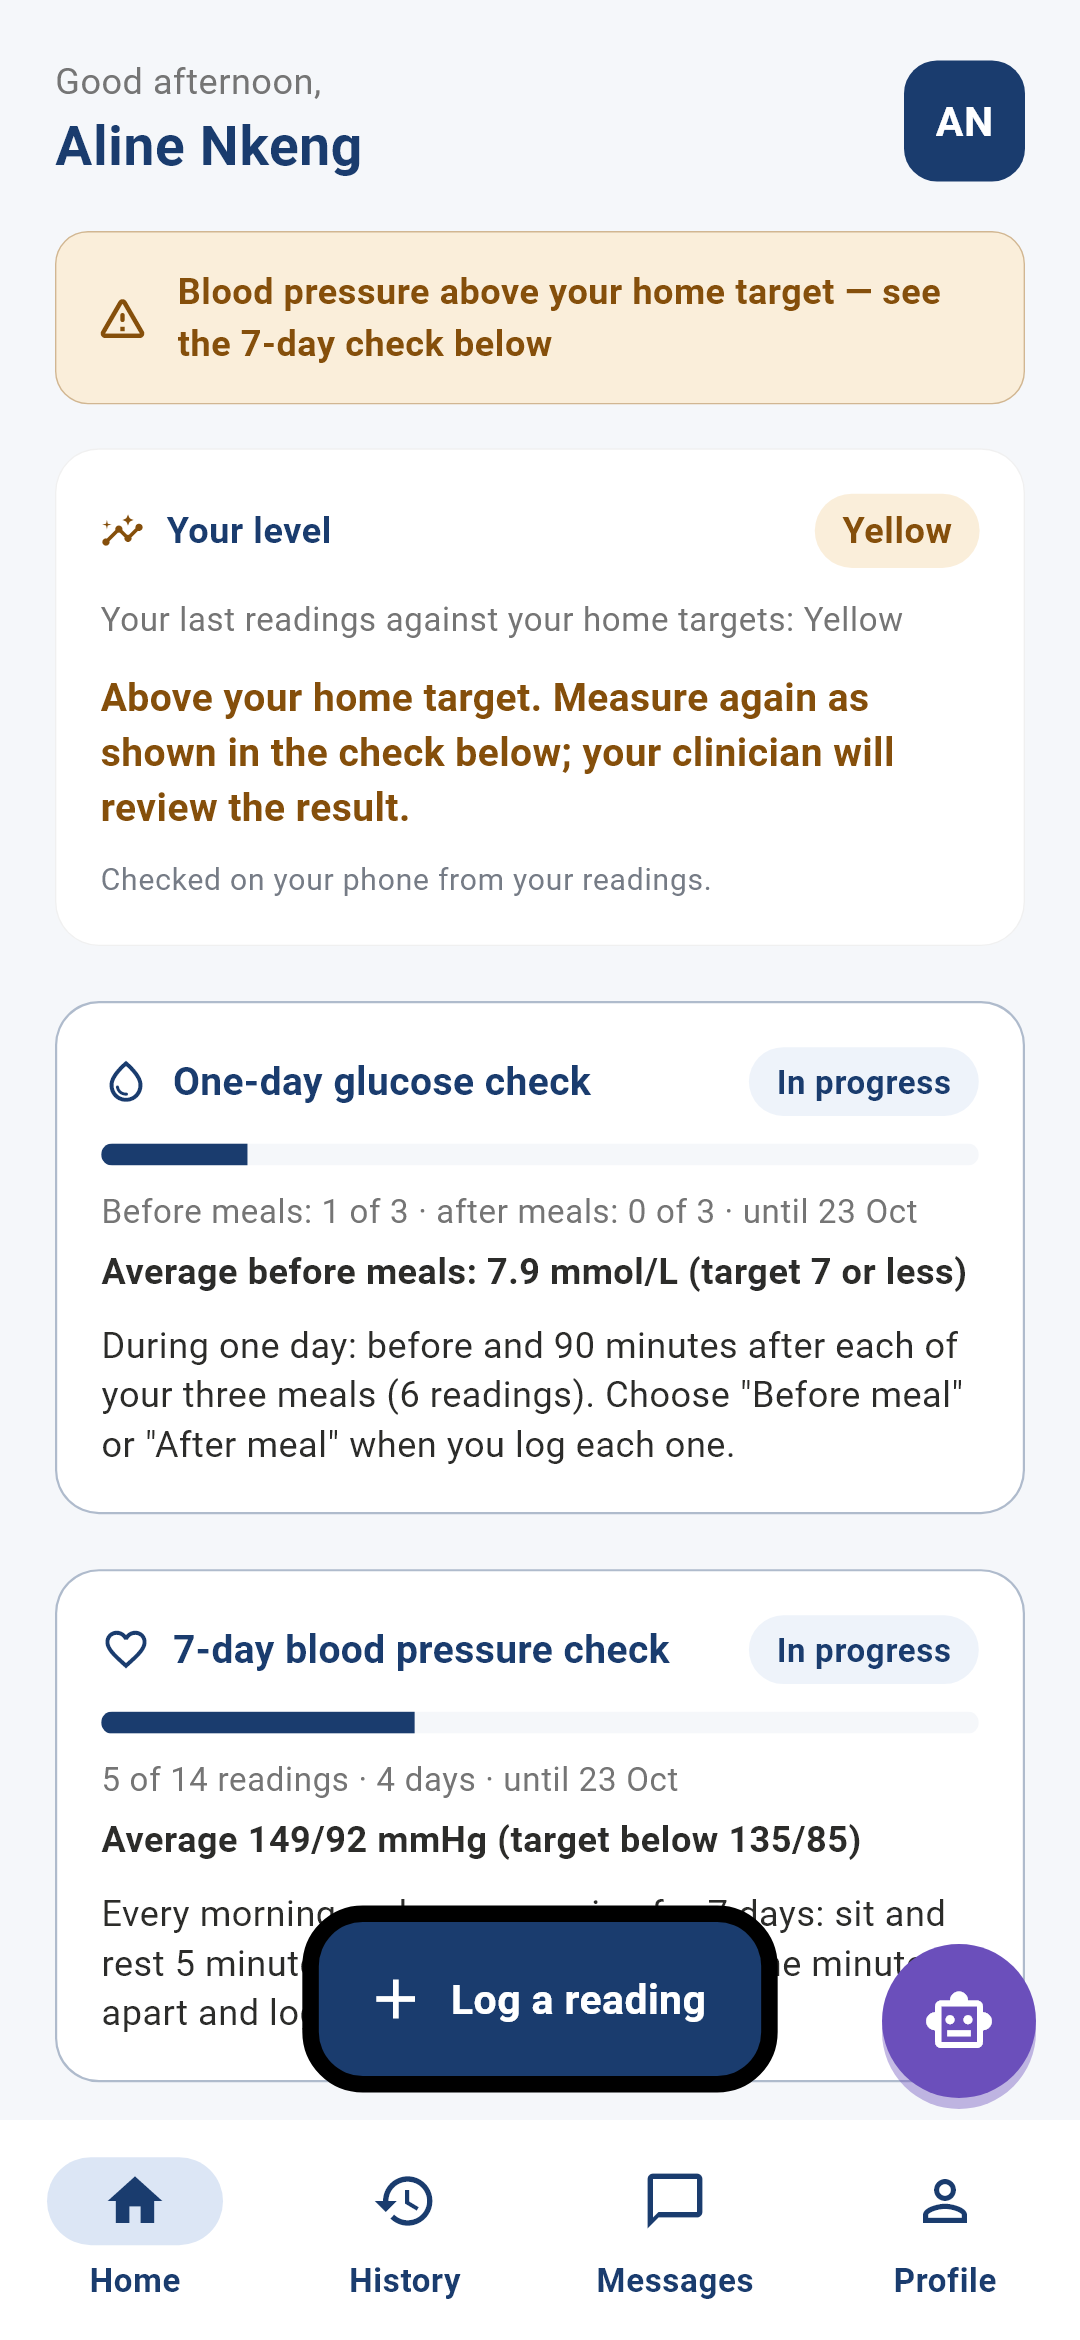
\includegraphics[width=\linewidth]{figures/screens/home_light.png}
  \caption{Patient home}
\end{subfigure}\hfill
\begin{subfigure}[t]{0.17\textwidth}\centering
  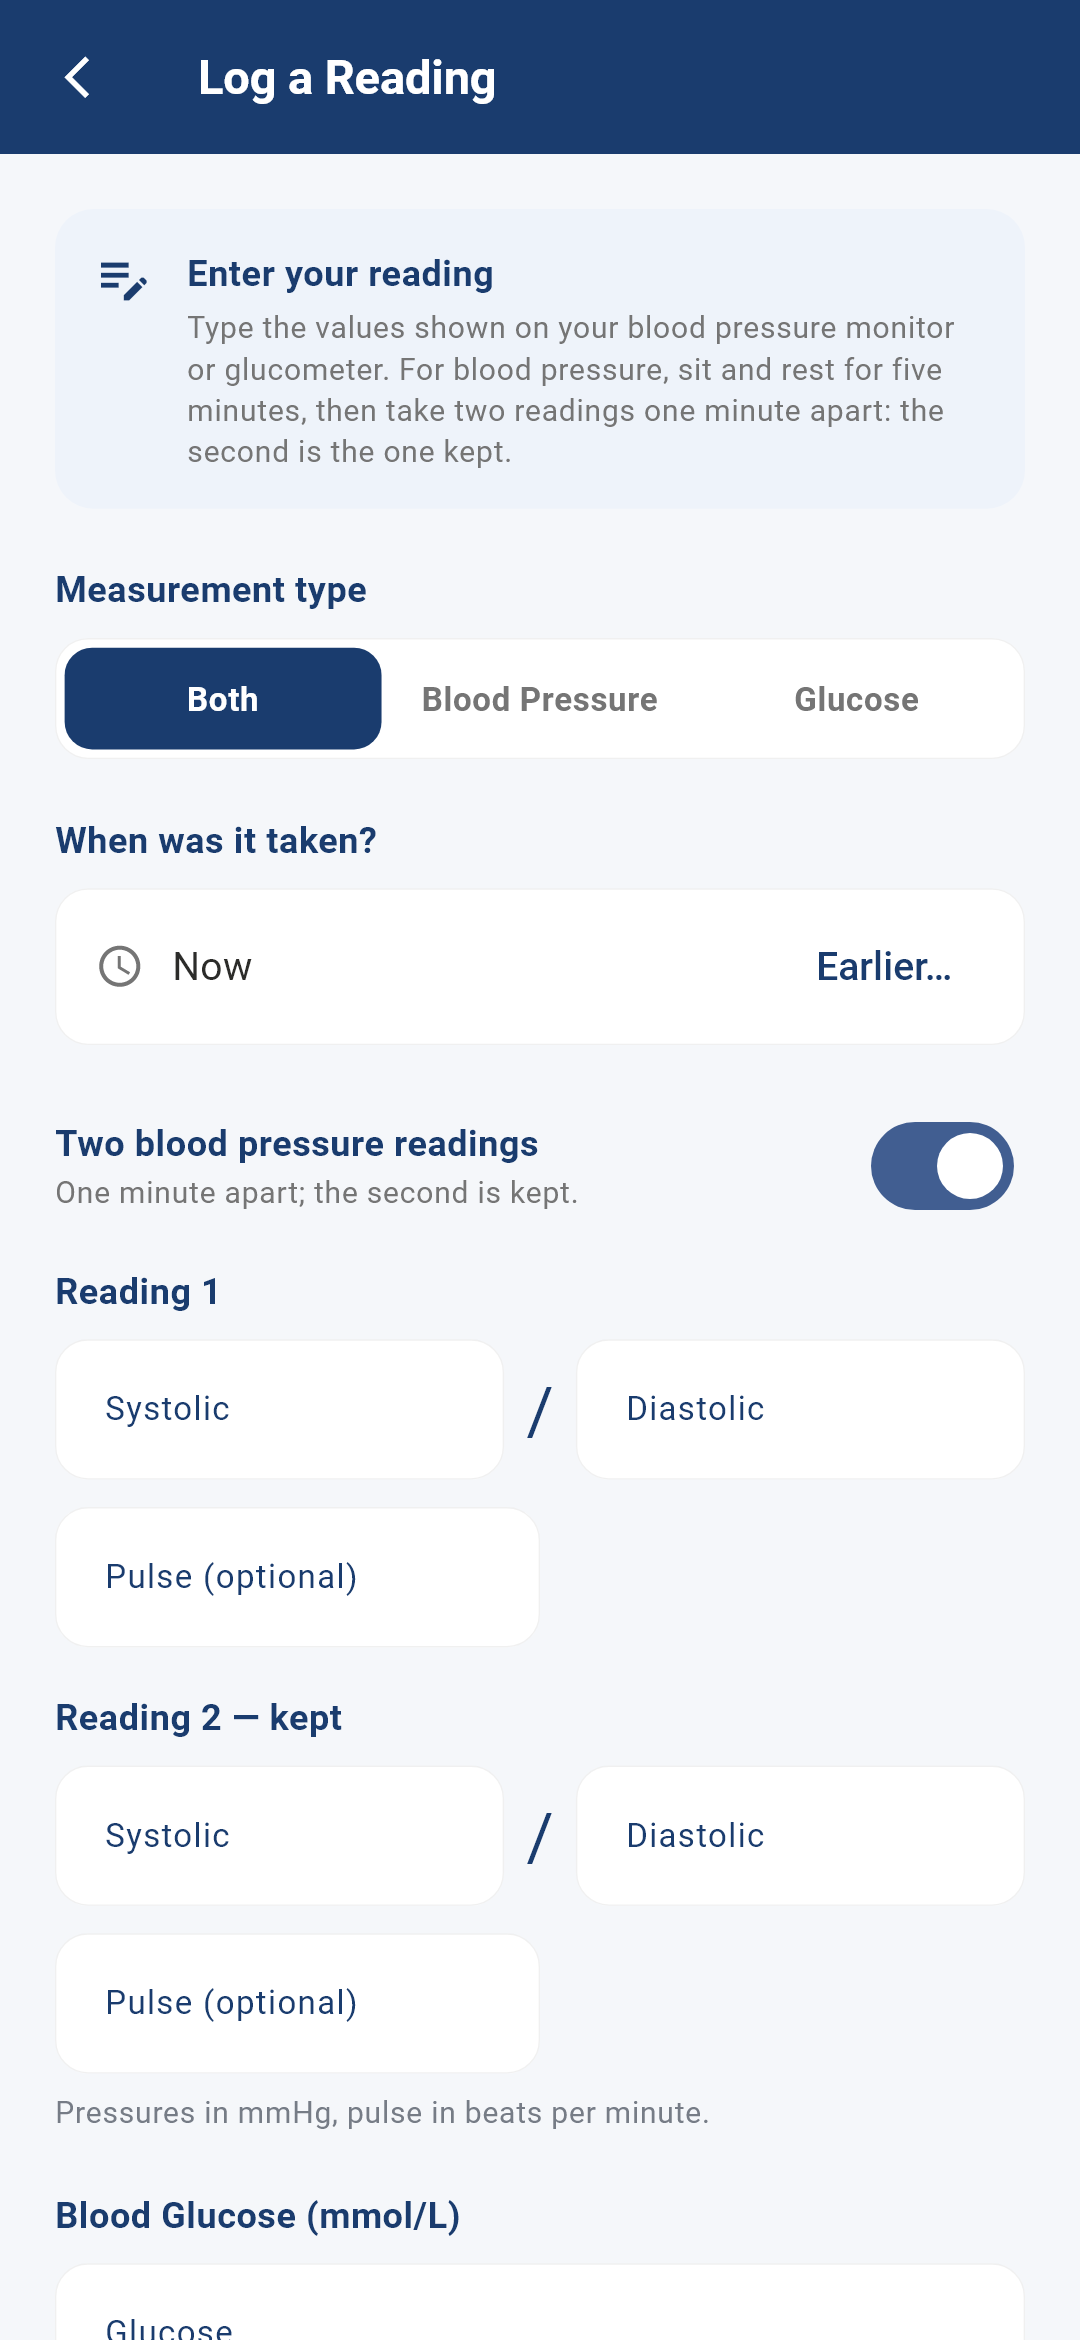
\includegraphics[width=\linewidth]{figures/screens/log_reading_light.png}
  \caption{New reading}
\end{subfigure}

\vspace{0.35cm}
\begin{subfigure}[t]{0.17\textwidth}\centering
  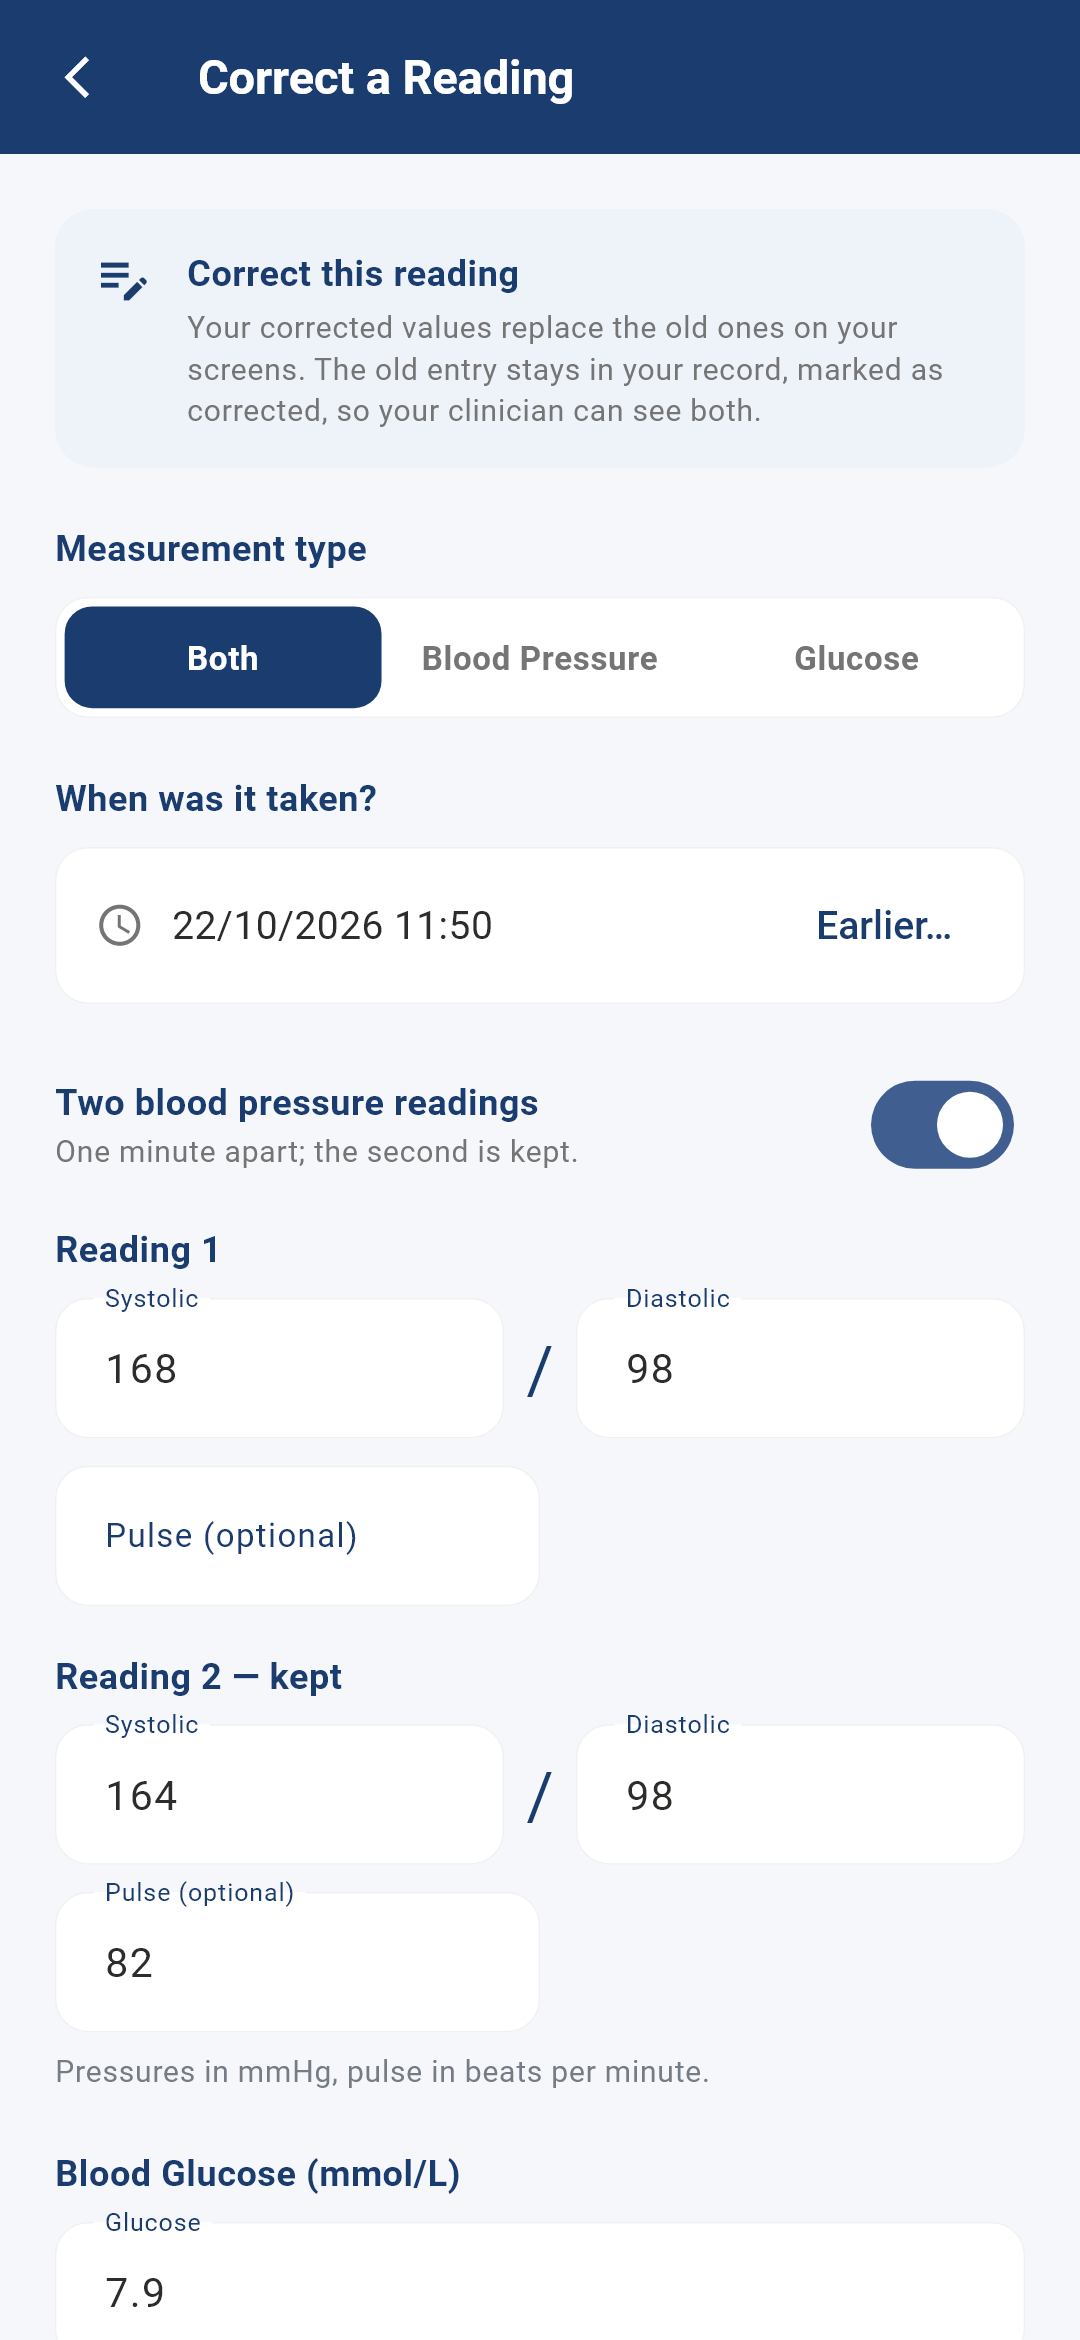
\includegraphics[width=\linewidth]{figures/screens/correct_reading_light.png}
  \caption{Correction}
\end{subfigure}\hfill
\begin{subfigure}[t]{0.17\textwidth}\centering
  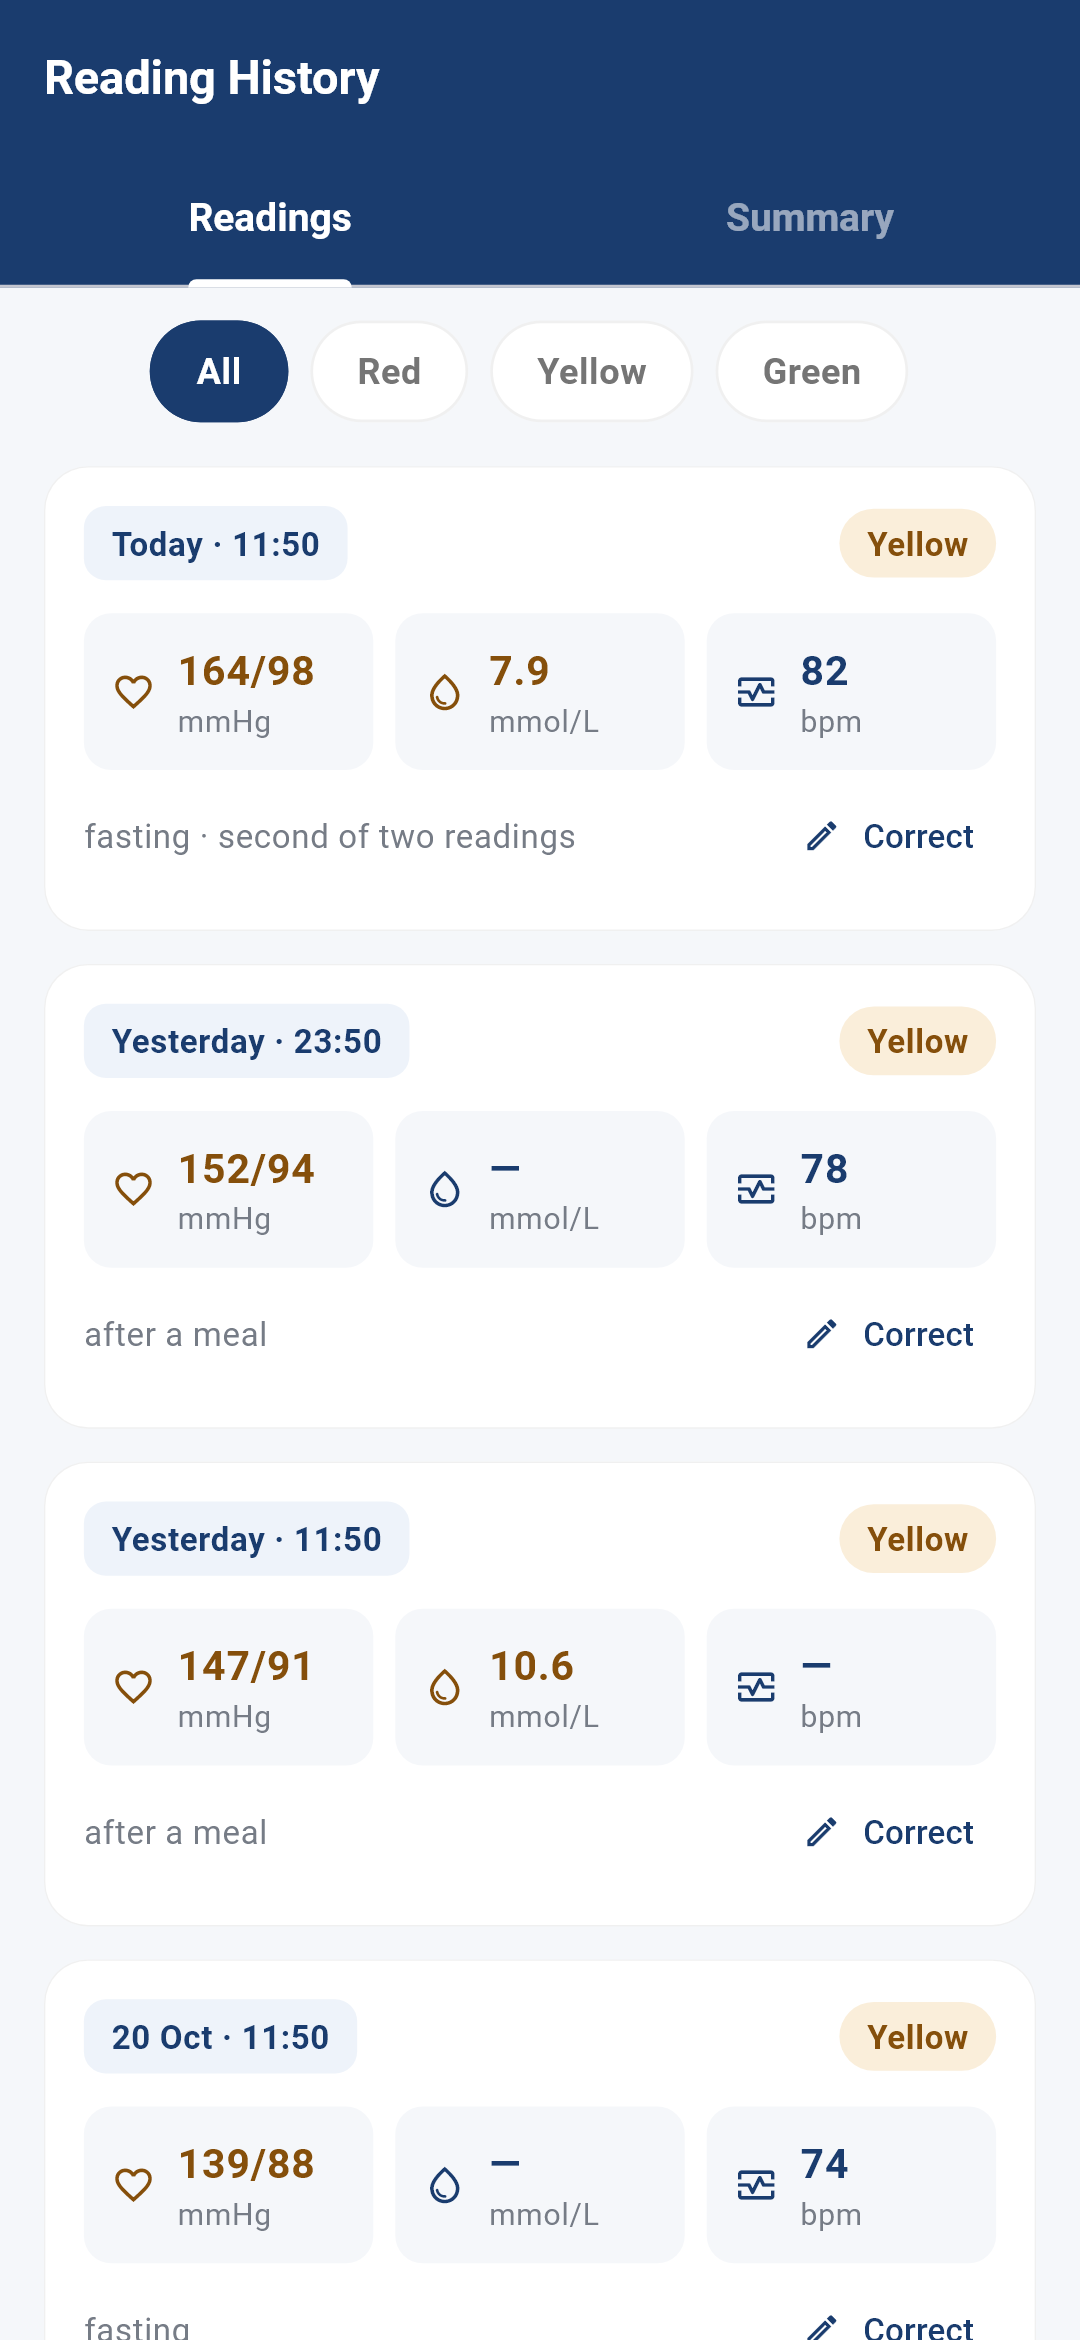
\includegraphics[width=\linewidth]{figures/screens/history_light.png}
  \caption{History}
\end{subfigure}\hfill
\begin{subfigure}[t]{0.17\textwidth}\centering
  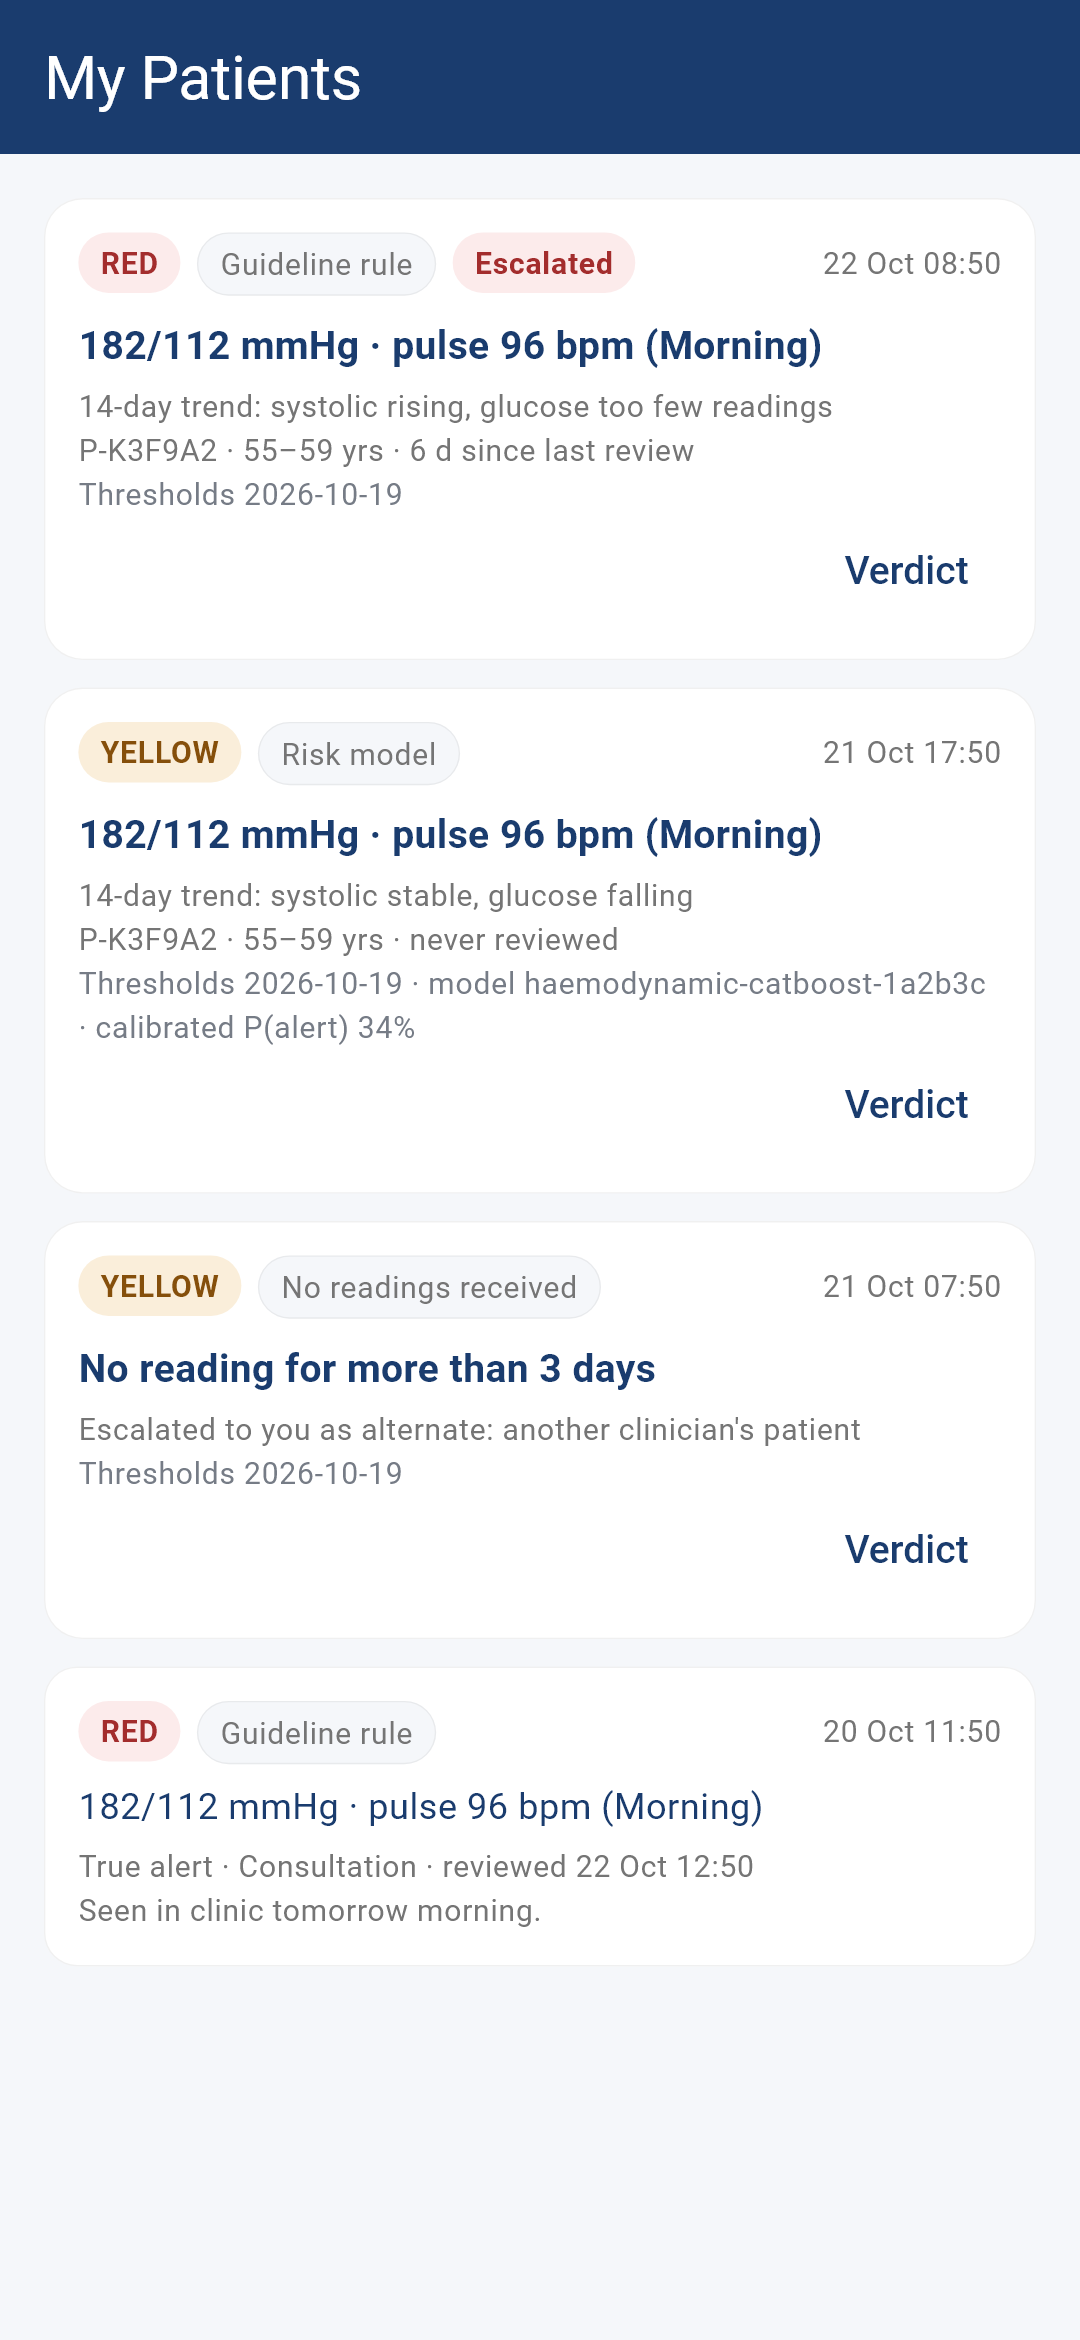
\includegraphics[width=\linewidth]{figures/screens/queue_light.png}
  \caption{Clinician queue}
\end{subfigure}\hfill
\begin{subfigure}[t]{0.17\textwidth}\centering
  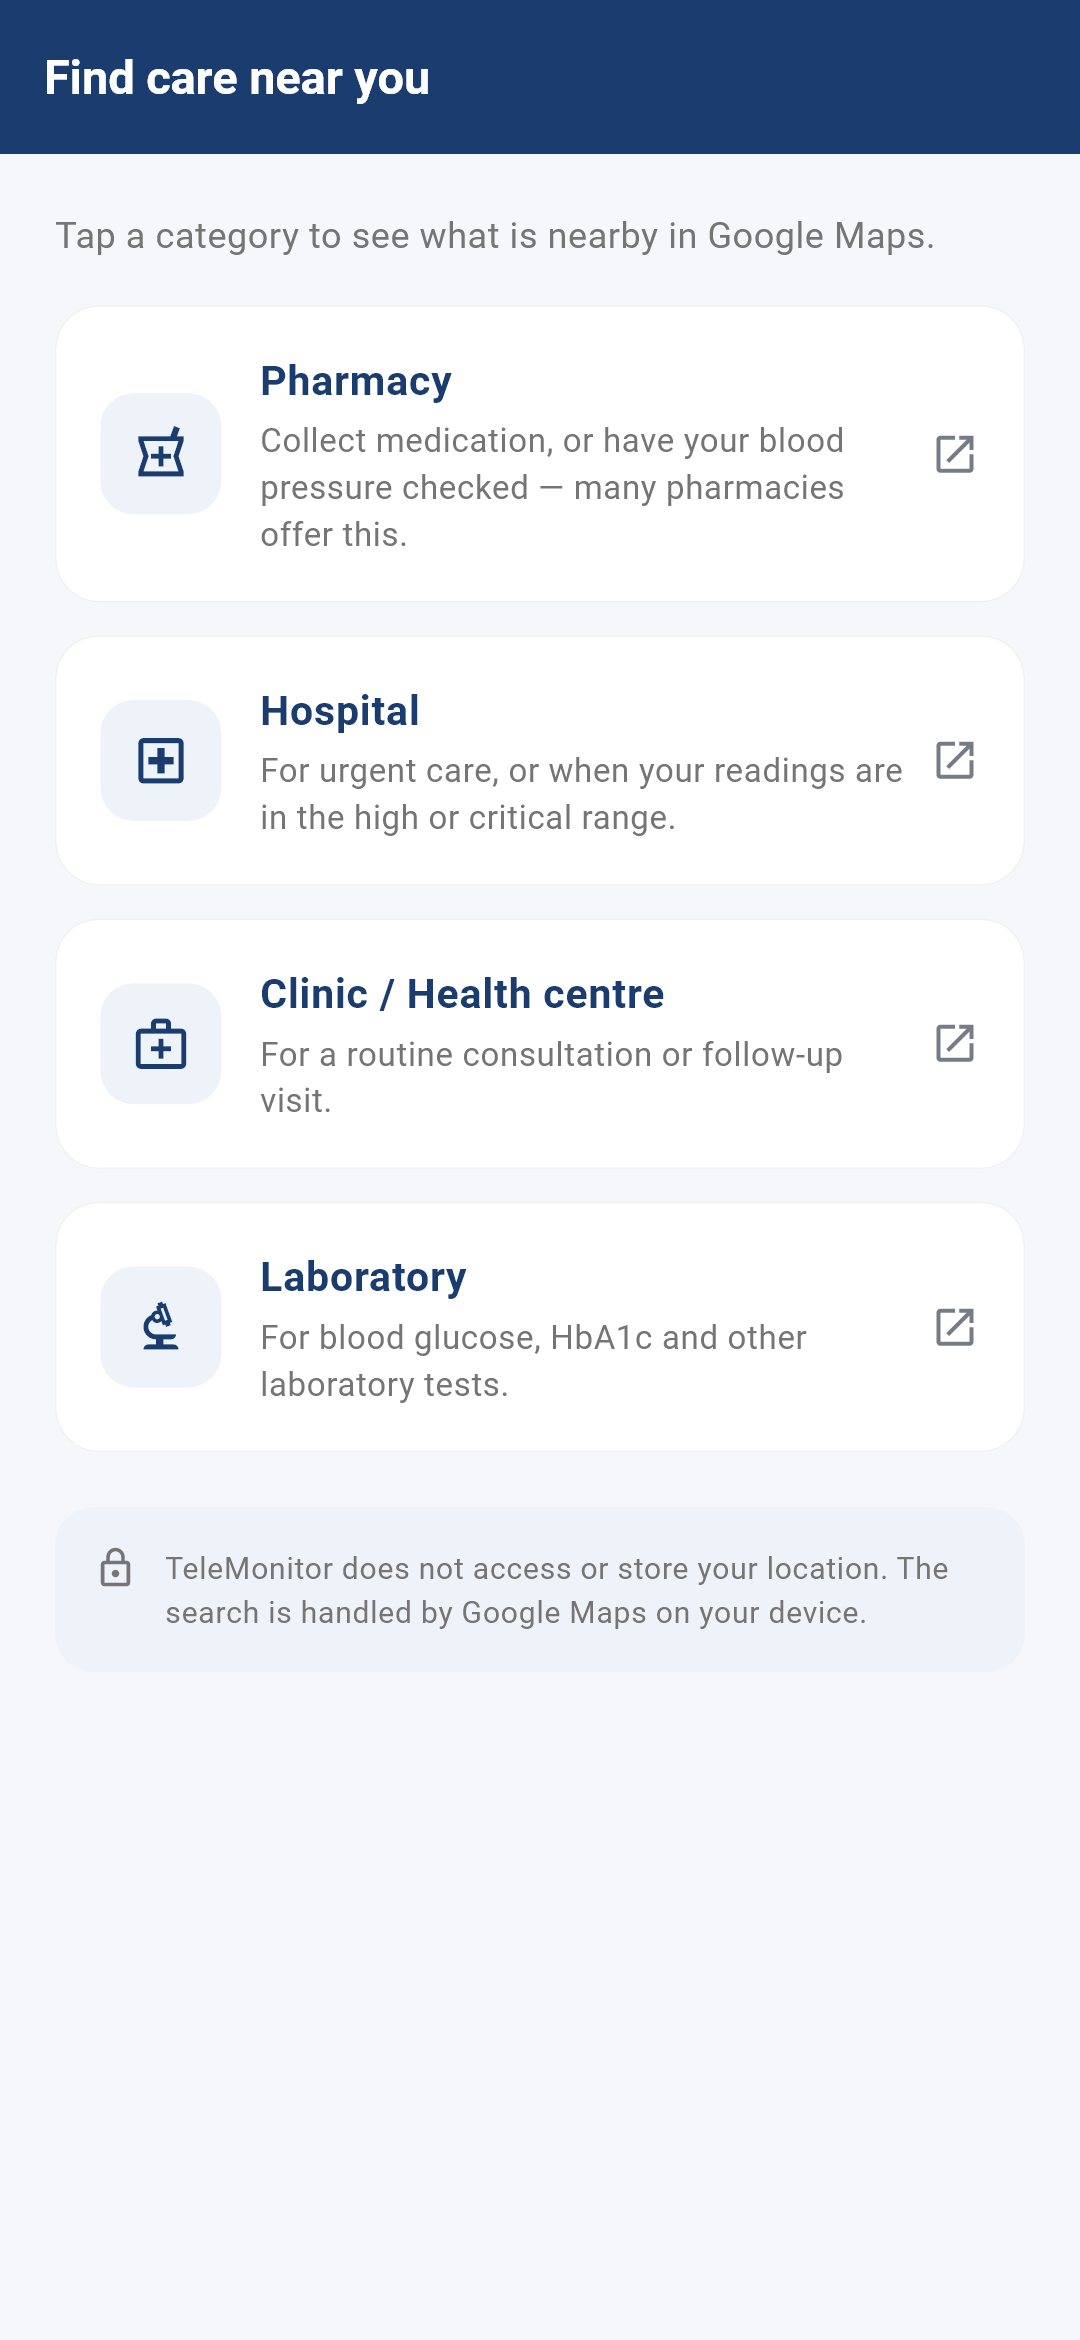
\includegraphics[width=\linewidth]{figures/screens/care_finder_light.png}
  \caption{Nearby care}
\end{subfigure}
\caption{Screens of the application: (a) sign-in, shared by patients and clinicians; (b) enrolment with the clinician's code; (c) patient home with the level, the instruction and the verification profiles; (d) entry of the two readings of the protocol; (e) correction, a new reading that supersedes the old one; (f) history with level and corrections; (g) clinician queue, red before yellow; (h) nearby care, opened in the phone's maps. Rendered by the widget tests with fictitious patients; model names and probabilities are test values.}\label{fig:screens}
\end{minipage}

\chapter{TRIPOD+AI Checklist}\label{app:tripod}

The modelling study is reported according to TRIPOD+AI \parencite{collins2024}; its risk of bias can be assessed with PROBAST+AI \parencite{moons2025}.

{\footnotesize
\begin{longtable}{@{}>{\raggedright\arraybackslash}p{1.1cm} >{\raggedright\arraybackslash}p{4.3cm} >{\raggedright\arraybackslash}p{8.6cm}@{}}
\caption{TRIPOD+AI items and where they are addressed.}\label{tab:tripod}\\
\toprule
\textbf{Item} & \textbf{Topic} & \textbf{Where} \\
\midrule
\endfirsthead
\toprule
\textbf{Item} & \textbf{Topic} & \textbf{Where} \\
\midrule
\endhead
1 & Title & title page \\
3a--c & Background, intended use, inequalities & Introduction; \cref{sec:lit-gaps} (Central Africa absent from the evidence) \\
4 & Objectives & Introduction (objectives, research questions, hypotheses) \\
5a--b & Data sources, dates & \cref{sec:data-collection}: Douala 2026; eICU 2014--2015; \cref{app:data} \\
6a--b & Setting, eligibility & \cref{sec:data-collection,sec:harmonisation}; \cref{app:data} \\
6c & Treatments & not recorded in either dataset \\
7 & Data preparation & \cref{sec:preprocessing} \\
8a--c & Outcome, assessment, blinding & \cref{sec:labelling}; blinded relabelling by the partner physician planned (100--150 readings), not yet done \\
9a--c & Predictors & \cref{sec:features}; instruments in \cref{sec:instruments-obtained} \\
10 & Sample size & \cref{sec:sampling,sec:results-sample-size} \\
11 & Missing data & \cref{sec:missingness} \\
12a--g & Partitioning, handling, model type, clusters, measures, updating, computation & \cref{sec:evaluation,sec:metrics,sec:ml,sec:tools}; outer folds by hospital; intercept update; \cref{app:config} \\
13 & Class imbalance & class weights and their correction (\cref{sec:evaluation}) \\
14 & Fairness & results by sex, age band and hospital (\cref{sec:results-benchmark}) \\
15 & Output, thresholds & \cref{sec:tiers} \\
16 & Development against evaluation data & \cref{sec:results-data} \\
17 & Ethical approval & \cref{sec:ethics-considerations} \\
18c--f & Protocol, registration, sharing & protocol fixed before results; not registered; \cref{sec:tools} \\
19 & Patient and public involvement & none \\
20--27 & Results, discussion & \cref{ch:results} \\
\bottomrule
\end{longtable}
}
